% HTML:
% htlatex tex4ht-final.tex "tex4ht-config" " -cunihtf -utf8"
%
% Para subir a GitHub duplicar  tex4ht-final.html y renombrarlo a index.html 

\documentclass[12pt,a4paper,twoside]{article}


\usepackage[utf8]{inputenx}
\usepackage[T1]{fontenc}

\usepackage{ifpdf}


%\usepackage[shorthands=off]{babeltools}
%\babelshorthand{:}
%\ifpdf
%	\usepackage[spanish]{babel} % conflicto con hyperref con tex4ht
%\else
%\fi
%\usepackage{lnspbabel}

\usepackage{parskip}
\usepackage{microtype}

\usepackage{amsmath}

\ifpdf
	\usepackage{graphicx}
\else
	\usepackage[dvipdfmx]{graphicx}
\fi


\usepackage{lipsum}

%\ifpdf
%\usepackage{hyperref}
%\hypersetup{colorlinks,linkcolor=green}
%\else
%\usepackage[colorlinks, dvips]{hyperref}
%\fi
%\usepackage{exerquiz}
%\usepackage[dvips]{exerquiz}
%\usepackage[dvips,colorlinks]{hyperref}
\RequirePackage{url}
\usepackage{lnhyperref}



\title{Practicando con \TeX4ht{}}
\author{Eva María Mazcuñán Navarro}

\begin{document}

\maketitle

\ifdefined\HCode
\else
	\tableofcontents
\fi



\section{Matemáticas}

\label{sec:math}

Veamos cómo se visualizan en el navegador:

\begin{itemize}
	\item las fórmulas delimitadas con dólares $1<x<2$, $x^2+y^2=9$ y $y=\sqrt{9-x^2}$
	
	\item las fórmulas delimitadas con paréntesis \(1\le x \le 2\), \(x^2+y^2=9\) y  \(y=\sqrt{9-x^2}\)
	
	\item la fórmula \[\int_a^b f(x)dx.\]
\end{itemize}

\section{Fuentes}

Comandos: Escritura en \textbf{\bfseries negrita}, \textit{\itshape itálica} y \textsf{\sffamily sans serif}.


Declaraciones: Escritura en {\bfseries negrita}, {\itshape itálica} y {\sffamily sans serif}.

Entornos: Escritura en \begin{bfseries}negrita\end{bfseries}, \begin{itshape} itálica \end{itshape} y  \begin{sffamily} sans serif \end{sffamily}.

Frase larga, para comprobar si se parte bien estupendamente  estupendamente  estupendamente. Frase larga, para comprobar si se parte bien estupendamente. Frase larga, para comprobar si se parte bien. Frase larga, para comprobar si se parte bien. Frase larga, para comprobar si se parte bien.

\section{Imágenes}

Sin escala:

\noindent Lorem ipsum dolor sit amet, consectetuer adipiscing elit. Lorem ipsum dolor sit amet, consectetuer adipiscing elit.\\
\noindent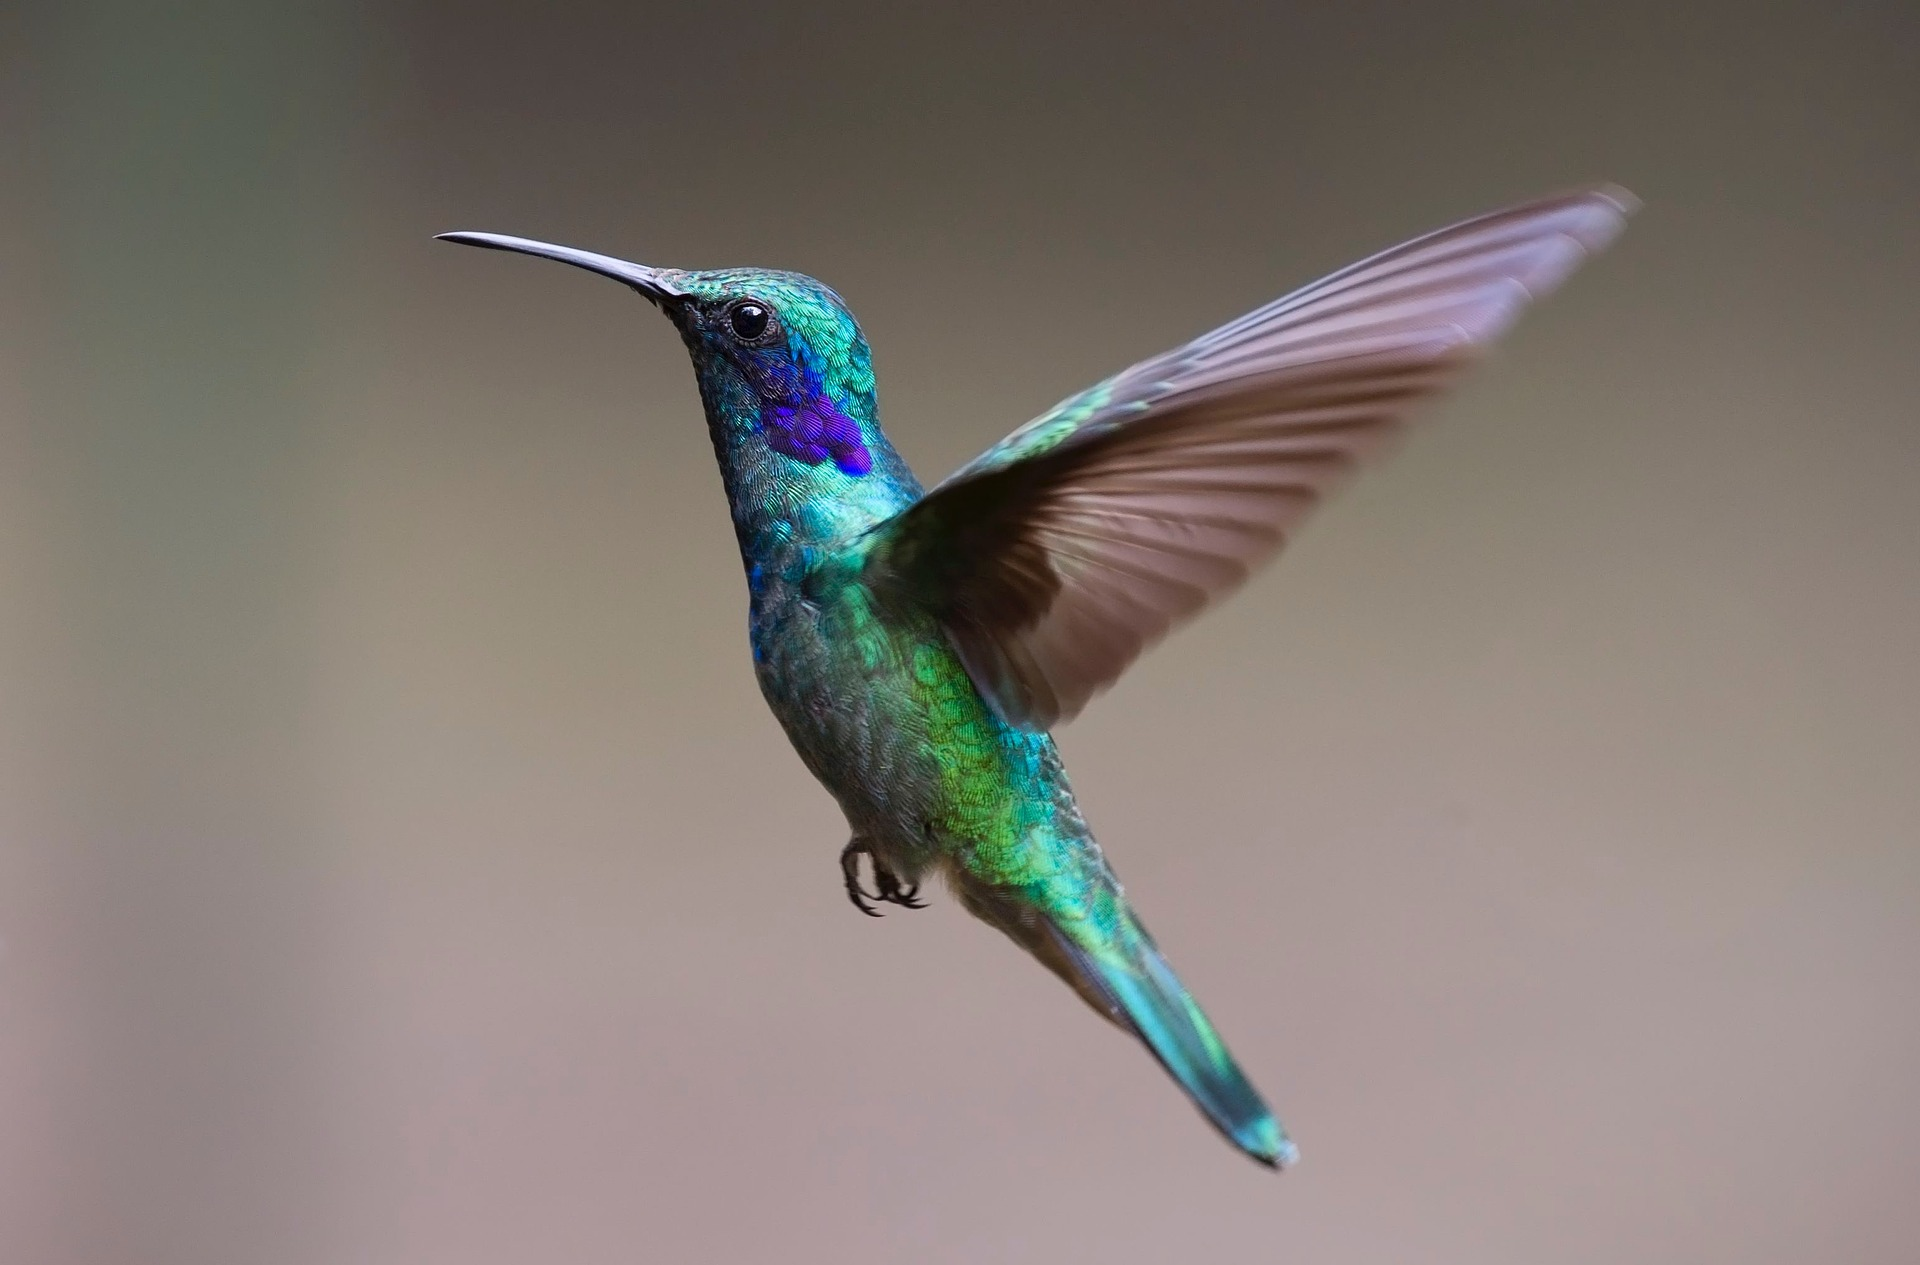
\includegraphics{images/bird.jpg}\\
\noindent Lorem ipsum dolor sit amet, consectetuer adipiscing elit. Lorem ipsum dolor sit amet, consectetuer adipiscing elit.\\
\noindent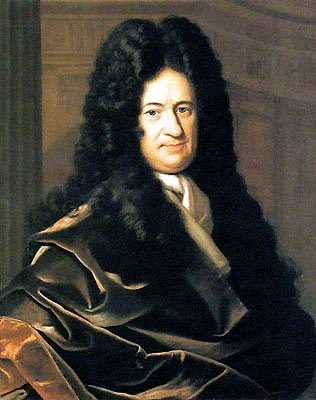
\includegraphics{images/GWLeibniz.png}

Escaladas a la mitad:

\noindent Lorem ipsum dolor sit amet, consectetuer adipiscing elit. Lorem ipsum dolor sit amet, consectetuer adipiscing elit.\\
\noindent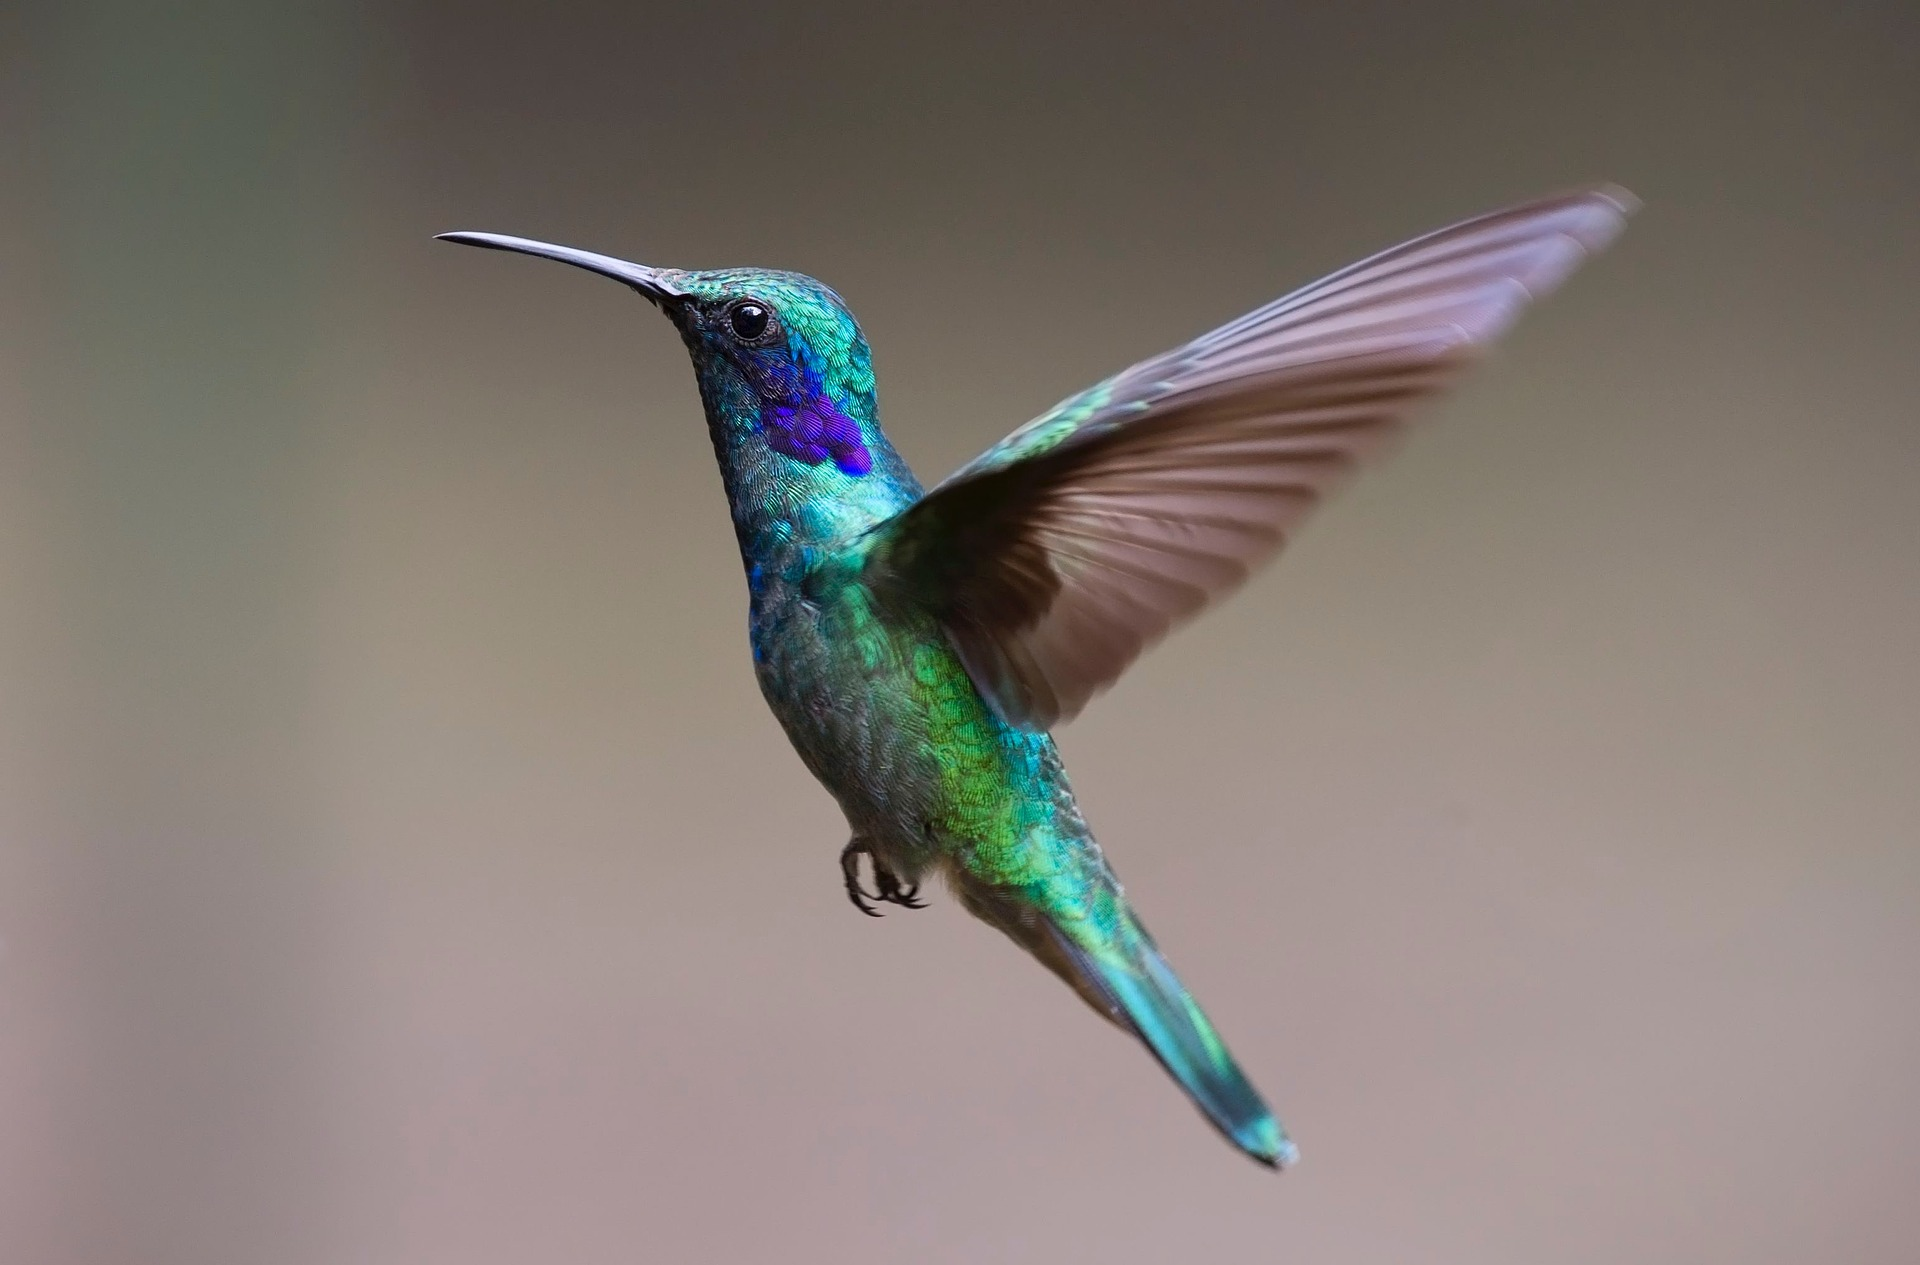
\includegraphics[scale=0.5]{images/bird.jpg}\\
\noindent Lorem ipsum dolor sit amet, consectetuer adipiscing elit. Lorem ipsum dolor sit amet, consectetuer adipiscing elit.\\
\noindent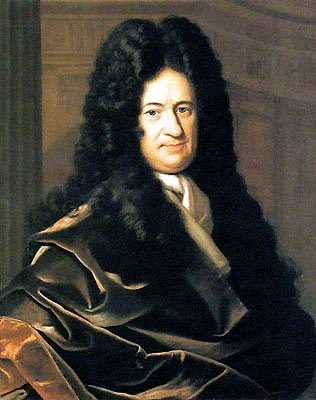
\includegraphics[scale=0.5]{images/GWLeibniz.png}

Anchura $40\%$ texto ($40\%$ de \the\dimexpr\textwidth\relax = \the\dimexpr .4\textwidth\relax):

\noindent Lorem ipsum dolor sit amet, consectetuer adipiscing elit. Lorem ipsum dolor sit amet, consectetuer adipiscing elit.\\
\noindent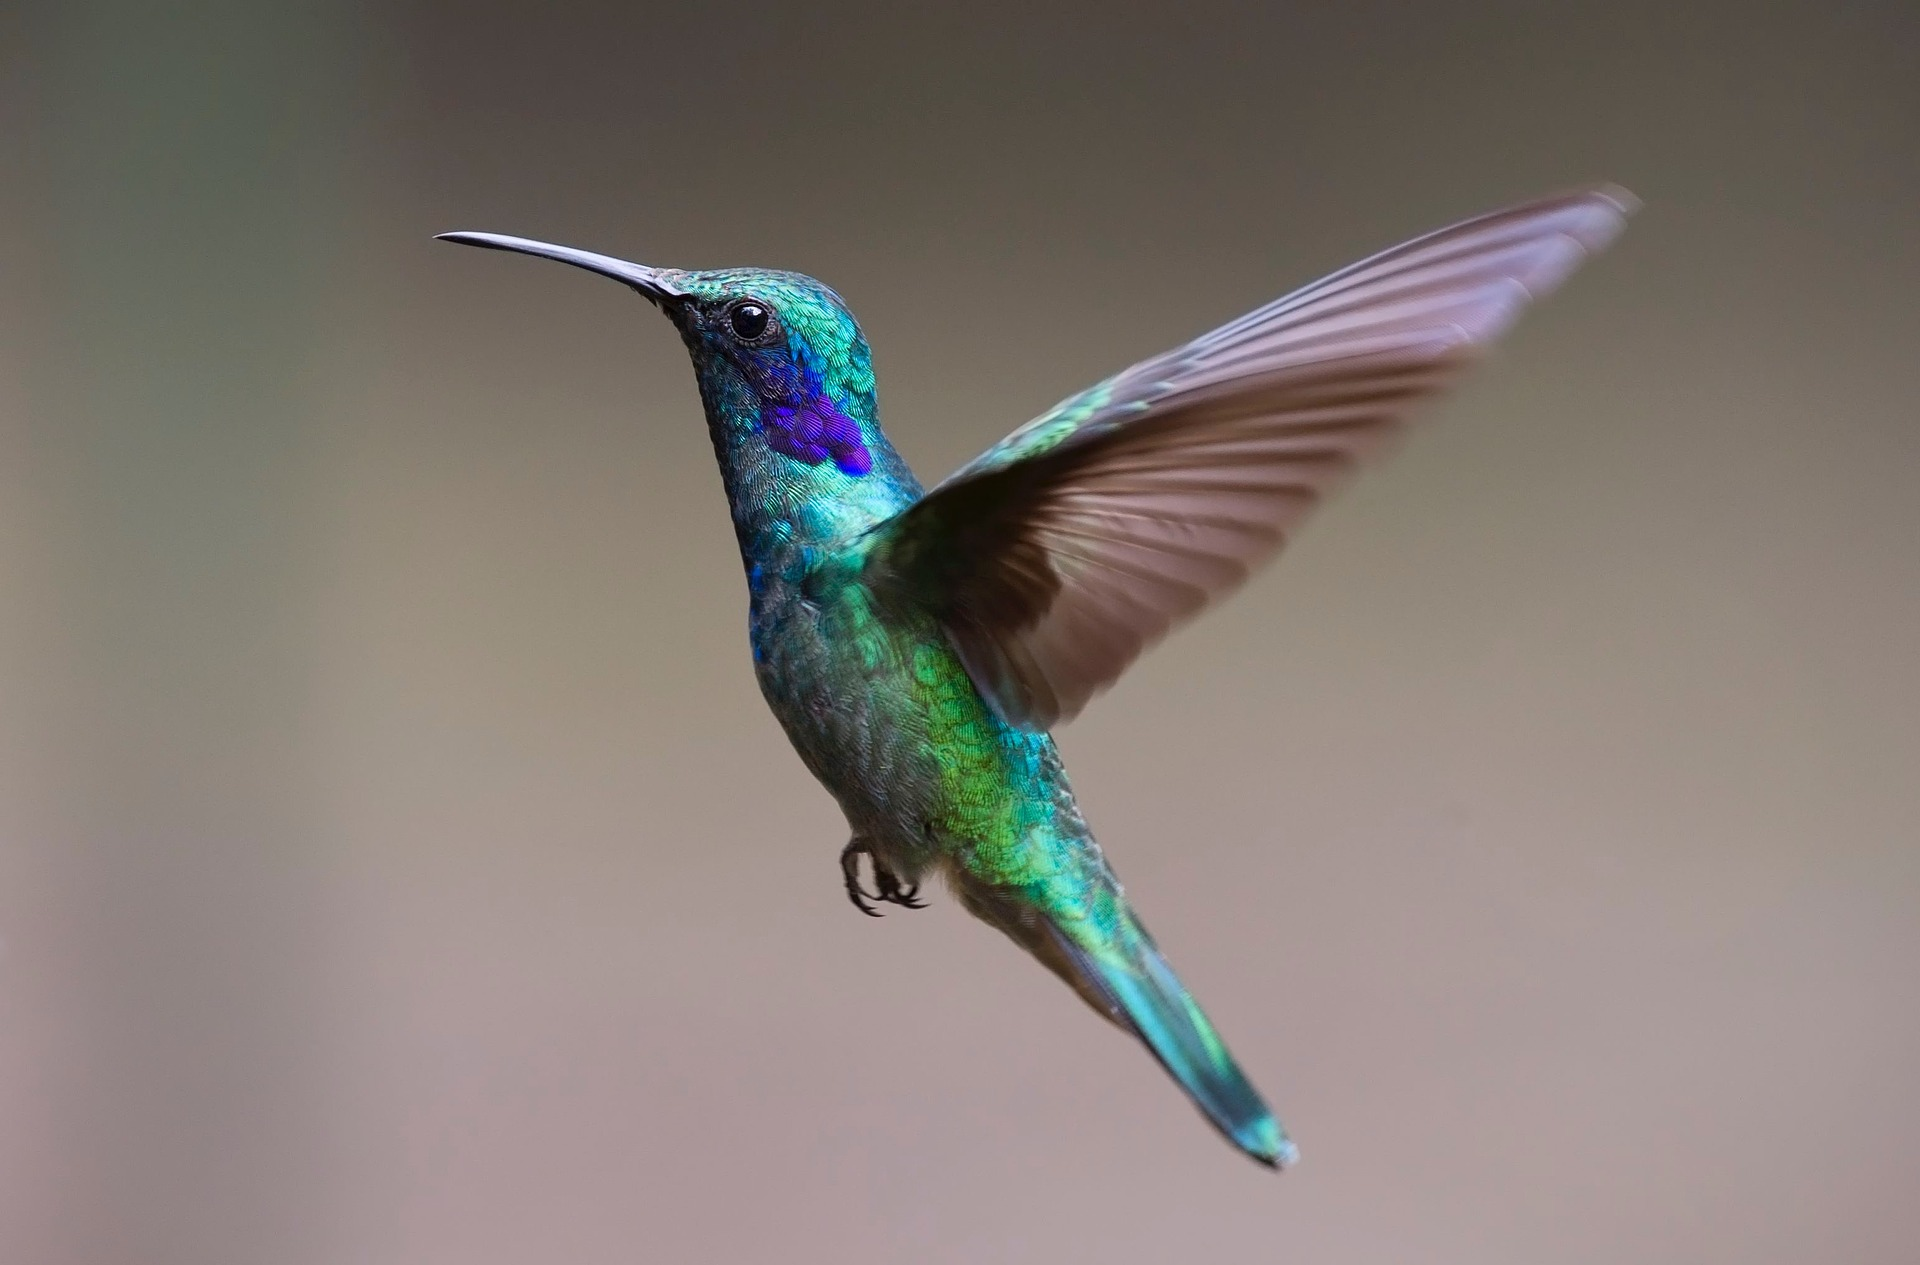
\includegraphics[width=.4\textwidth]{images/bird.jpg}\\
\noindent Lorem ipsum dolor sit amet, consectetuer adipiscing elit. Lorem ipsum dolor sit amet, consectetuer adipiscing elit.\\
\noindent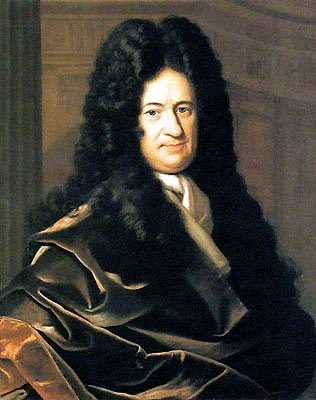
\includegraphics[width=.4\textwidth]{images/GWLeibniz.png}


%Anchura $40\%$ línea:
%
%\noindent Lorem ipsum dolor sit amet, consectetuer adipiscing elit.\\
%\noindent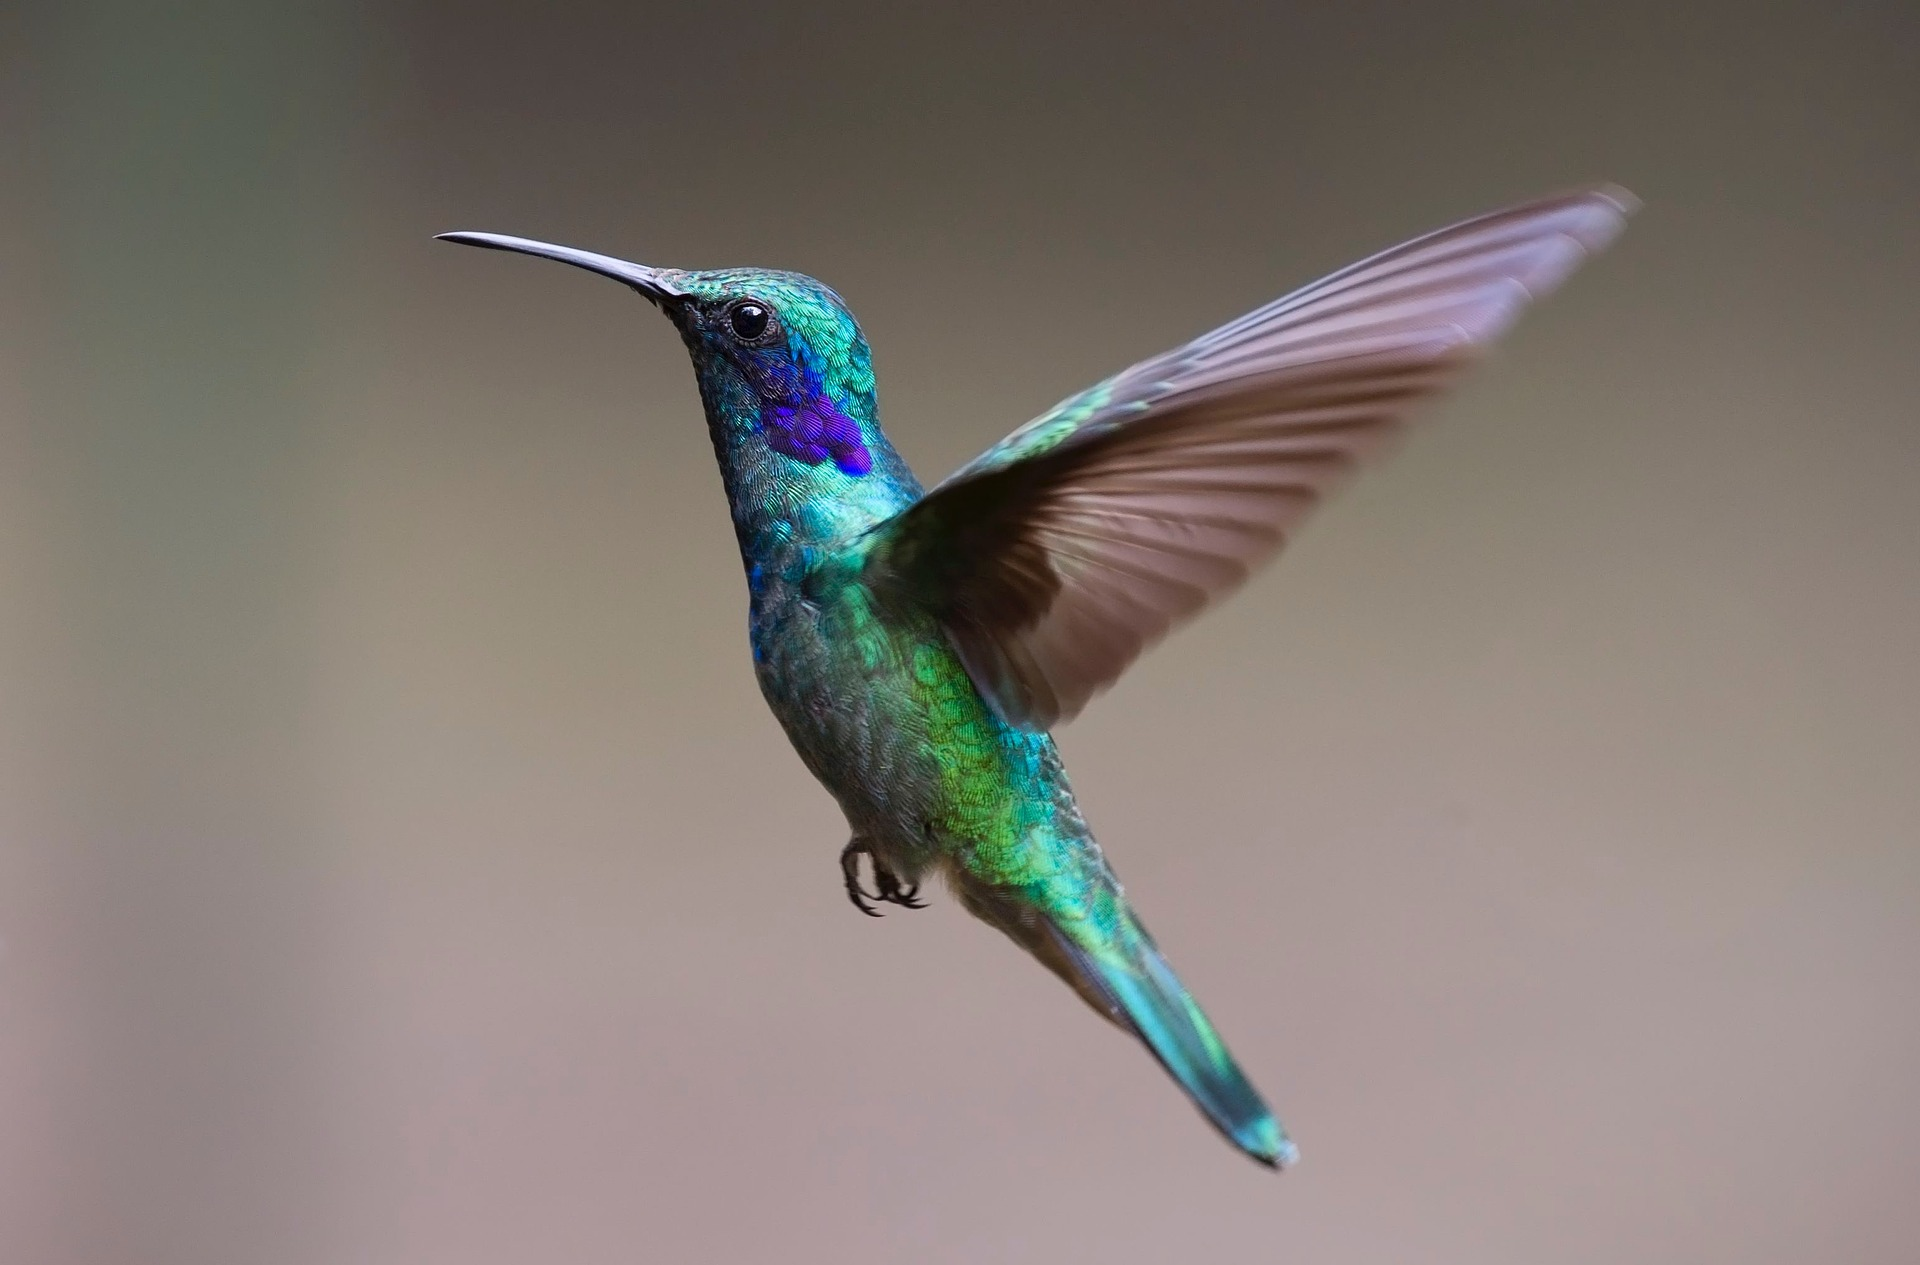
\includegraphics[width=.4\linewidth]{images/bird.jpg}\\
%\noindent Lorem ipsum dolor sit amet, consectetuer adipiscing elit.\\
%\noindent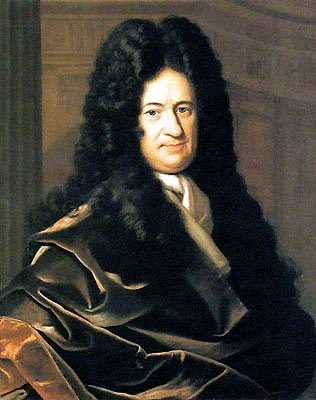
\includegraphics[width=.4\linewidth]{images/GWLeibniz.png}


Anchura 156pt:

\noindent Lorem ipsum dolor sit amet, consectetuer adipiscing elit.\\
\noindent\rule[2mm]{156pt}{3mm}\\
\noindent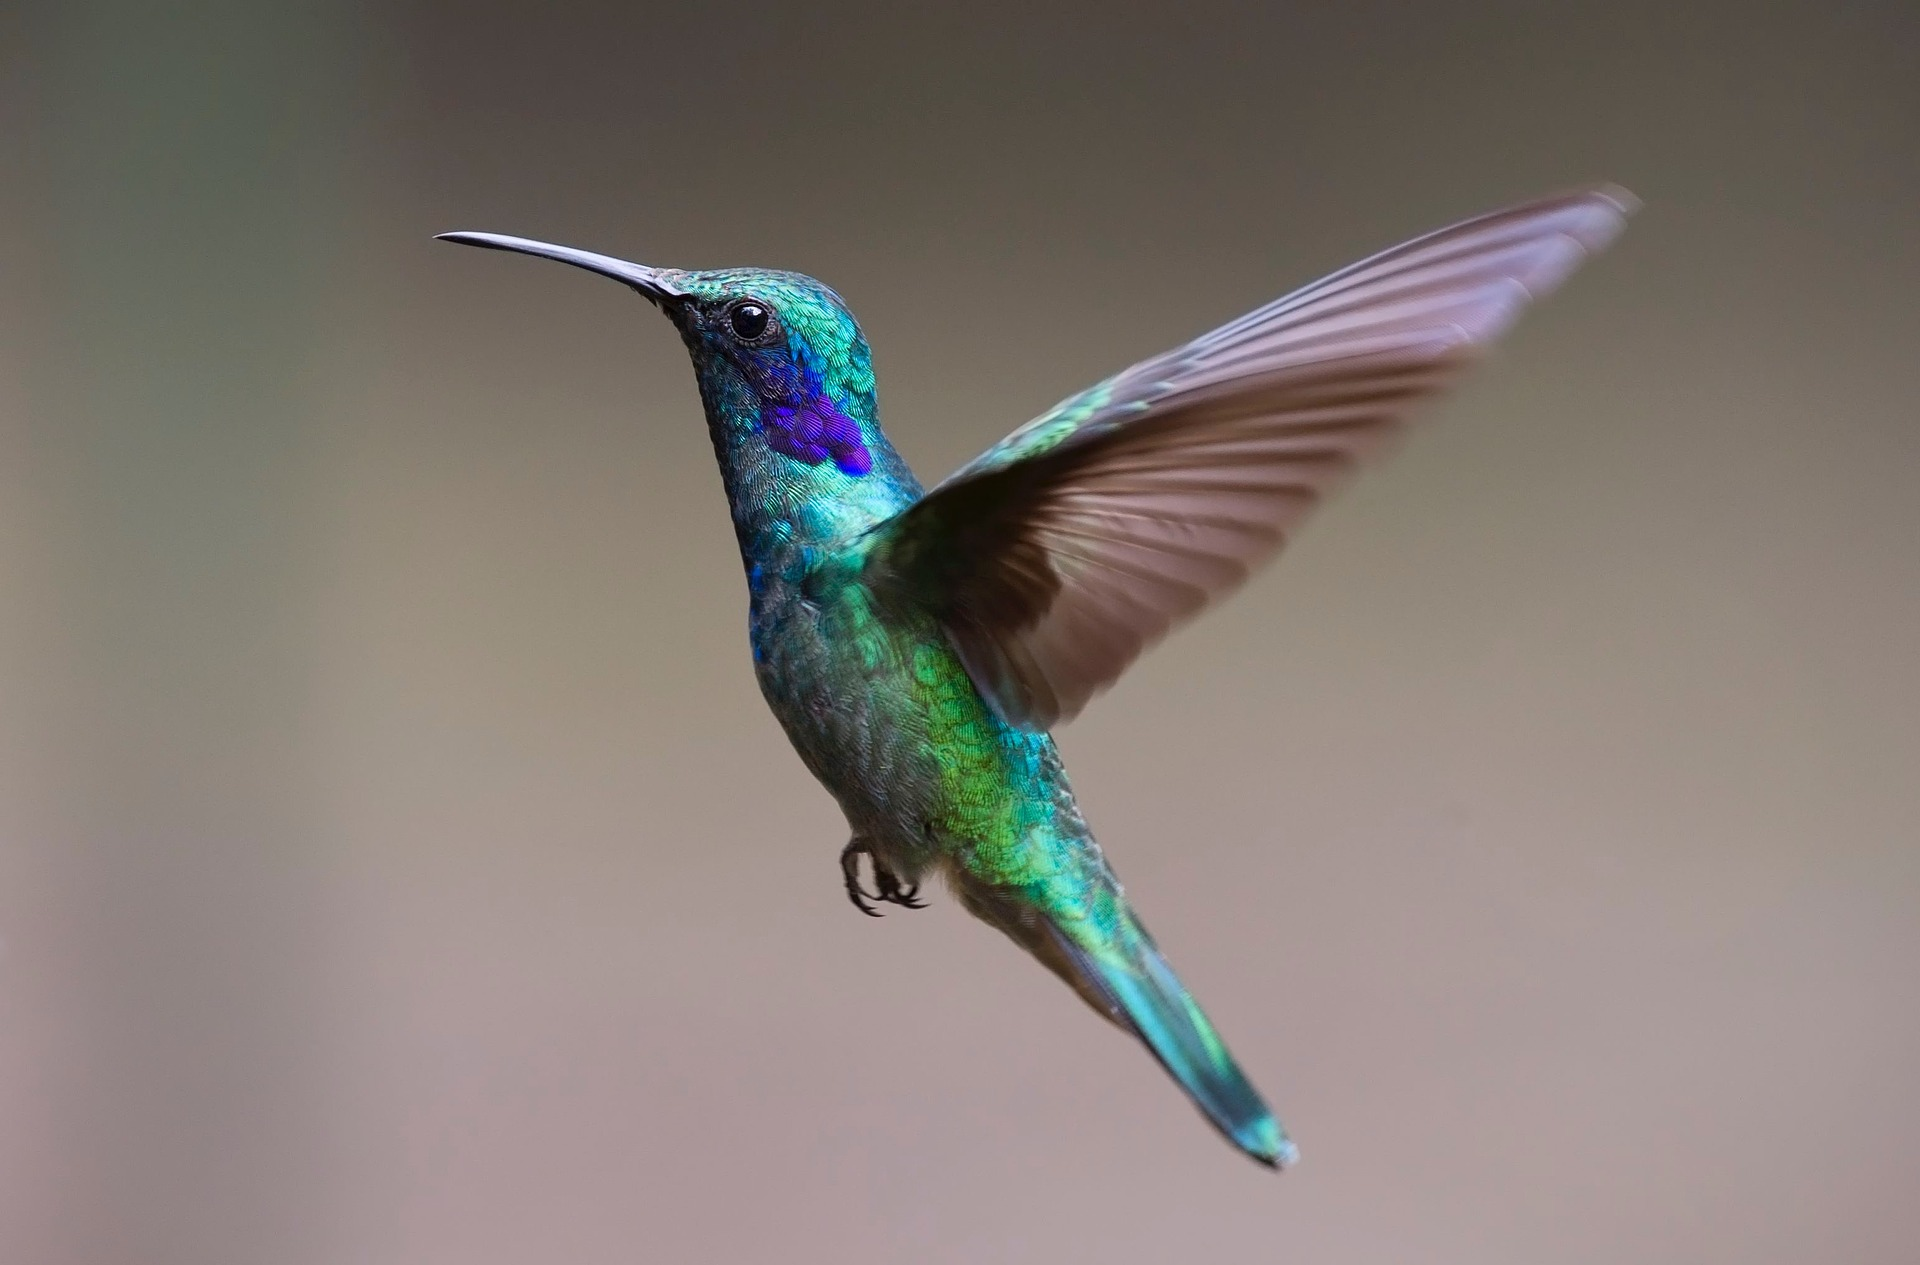
\includegraphics[width=156pt]{images/bird.jpg}\\
\noindent Lorem ipsum dolor sit amet, consectetuer adipiscing elit.\\
\noindent\rule[1em]{156pt}{1em}\\
\noindent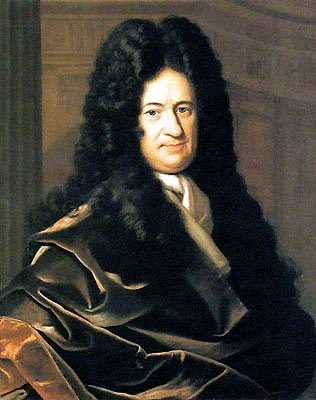
\includegraphics[width=156pt]{images/GWLeibniz.png}

\section{Hyperref}

En la sección \ref{sec:math} 
Visitar \href{https://edx.org}{pagina de EdX}
Visitar \href{https://edx.org}{pagina de EdX bla bla bla bla bla bla bla bla bla bla bla}

\section{exerquiz}
%
%
%\begin{shortquiz} % begin shortquiz environment
%Which of the following is the $\dfrac{d}{dx}{\sin(x^3)}$?
%\begin{answers}{4} % 4 columns of answers
%\Ans0 $\sin(3x^2)$ & % \Ans0 is a false answer
%\Ans0 $\cos(x^3)$ &
%\Ans1 $3x^2\cos(x^3)$ & % \Ans1 is the correct answer
%\Ans0 $3xˆ2\cos(3x^2)$
%\end{answers} % end answers environment
%\end{shortquiz} % end shortquiz environment
%
%
%\begin{shortquiz*}[KublaKhan1]
%Was it in Xanadu did Kubla Kahn a stately pleasure dome decree?
%\begin{answers}{4}
%\Ans1 True  & \Ans0 False
%\end{answers}
%\end{shortquiz*}

\section{Sección de relleno}

\lipsum[1-15]

\subsection{Subsección}

\lipsum[1-15]

\subsection{Otra subsección}

\lipsum[1-15]		

\section{Otra sección de relleno}

\lipsum[1-15]		

\section{Una última sección de relleno con el título muy largo muy largo muy largo}

\lipsum[1-15]

\end{document}